\section{DynSem Evaluation Backend}
\label{sec:dynsem-eval-strat}
An implementation for the \texttt{IEvaluationStrategy} as discussed in
\cref{sec:eval-strat} is made for languages that specify their dynamic
semantics using DynSem. The implementation class, called
\texttt{DynSemEvaluationStrategy} (see \cref{fig:uml-dynsem-eval-strat}),
evaluates REPL-specific DynSem rules and maintains the environment in which
evaluation takes place.

This section first goes over the configuration interface for DynSem that is
provided by the REPL. After that, the implementation of DynSem and of the
\texttt{DynSemEvaluationStrategy} are discussed in more detail.

\subsection{The configuration interface}
\label{sec:impl-repl-spec}
To evaluate a program in their language within the REPL, the language designer
has to make two kinds of configurations for the REPL in their DynSem
specification. The first is a rule for initializing the execution environment
for the REPL, shown in \cref{lst:shell-init}. The second are the rules for
implementing the REPL-specific semantics as discussed in
\cref{ssec:repl-spec-semant}.

\paragraph{Environment initialization} The initialization rule shown in
\cref{lst:shell-init} is evaluated upon the initialization of the evaluation
strategy. It instantiates the semantic components that form the execution
environment for the REPL: an environment with an initial variable binding of
$x \mapsto 4$, and an empty store. The evaluation strategy uses this in its
successive evaluations, and updates the execution environment after each result.

\begin{minipage}{\textwidth}
\begin{lstlisting}[language=dynsem,caption={The initialization rule for the
semantic components.},label={lst:shell-init},numbers=left]
rules
  // Initialization of shell state: an environment with "x" bound to 4,
  // and an empty store.
  ShellInit() -init-> ShellInit() :: Env { "x" |--> NumV(4) }, Store {}.
\end{lstlisting}
\end{minipage}

\paragraph{REPL-specific semantics} The second kind of configuration are the
rules for the REPL-specific semantics. These can be seen as entry points for the
REPL to the interpreter. The rules are all named ``shell'', so that they are
distinct of the ordinary semantics. \Cref{lst:shell-rule} shows an example of
such a rule. The rule implements a construct that is only valid when evaluating
within the REPL: it implements binding the result of an expression to a
variable. With the specification of this rule, the bound variable can be used in
successive evaluations done by the user.

Note that the environment \textit{E} is passed as a read-write component,
instead of a read-only component as is explained in \cref{ssec:dynsem}. This is
because in this case the environment \emph{should} be writable, since the
resulting environment after execution should be available to the REPL. Note also
that in line 5 of the rule, the rest of the specification is recursively
invoked. This shows that much of the existing specification can be reused when
implementing the REPL-specific semantics.

\begin{minipage}{\textwidth}
\begin{lstlisting}[language=dynsem,caption={A rule specifying semantics specific
to the REPL.},label={lst:shell-rule},numbers=left]
rules
  // let x = 2
  Let(x, e) :: E -shell-> v :: E'
  where
    E |- e :: Store {} --> v :: Store _;
    E |- bindVar(x, v) --> E'.
\end{lstlisting}
\end{minipage}

\subsection{The implementation}
\label{ssec:implementation}
This section discusses the implementation of the evaluation
strategy. However, before doing this, an explanation of the interfaces provided
by DynSem and its generated interpreters is in order.

\paragraph{DynSem's generated interpreters} As explained in \cref{ssec:dynsem},
DynSem is able to generate interpreters in Java from a dynamic semantics
specification written in the DynSem meta-language. DynSem uses the Truffle
language implementation framework for its generated
interpreters~\cite{Humer14}. By using the Truffle framework, the generated
interpreter can benefit from the performance optimizations of the Truffle
virtual machine (VM)~\cite{Wurthinger13}, as opposed to writing one's own
optimizations instead.

The evaluation of a program is done by invoking a reduction rule with as its
arguments the program in the form of an AST, and the semantic components. A
reduction rule can be found by performing a lookup with the rule's signature as
the lookup key, through Truffle's foreign object access
interface~\cite{Grimmer15}. That is, the foreign objects are precisely the rules
such as the one shown in \cref{lst:shell-rule} (in the form of an internal
representation).

For this reason, the interpreter generated by DynSem can be seen as a
\textit{meta-interpreter}: it interprets a DynSem specification, and allows
access to rules as value objects through Truffle's foreign object access
interface. The rules themselves (or the ``values'' interpreted by the
meta-interpreter) can then be seen as access points to the interpreter of the
language, as they can be invoked with an AST and semantic components. The
relation between a meta-interpreter and an ordinary interpreter is captured in
the diagram shown in \cref{fig:meta-interpreter}.

\begin{figure}[b]
  \centering
  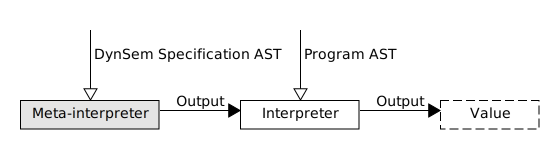
\includegraphics[width=0.8\textwidth]{meta-interpreter}
  \caption{The relation between a meta-interpreter and an ordinary interpreter.}
  \label{fig:meta-interpreter}
\end{figure}

\paragraph{The implementation of the evaluation strategy} The UML diagram of the
evaluation strategy is shown in \cref{fig:uml-dynsem-eval-strat}. The
\texttt{DynSemEvaluationStrategy} uses an \texttt{IInterpreterLoader} to
load the interpreter as generated by DynSem. It initializes the Truffle VM,
called the \texttt{PolyglotEngine}, with the interpreter generated by
DynSem, by evaluating the DynSem specification through the \texttt{eval} method
provided by the \texttt{PolyglotEngine}.

The \texttt{PolyglotEngine} provides the \texttt{findGlobalSymbol}
method, allowing the evaluation strategy to lookup the reduction rules of the
interpreter represented as a \texttt{Value} object. The returned
\texttt{Value} object has an \texttt{execute} method, which provides the
interface for invoking the reduction rule with the program AST and the semantic
components. This way, the configuration interface as outlined in
\cref{sec:impl-repl-spec} can be implemented: the initialization rule and the
REPL-specific rules can simply be looked up by their rule signature.

\begin{figure}[t]
  \centering
  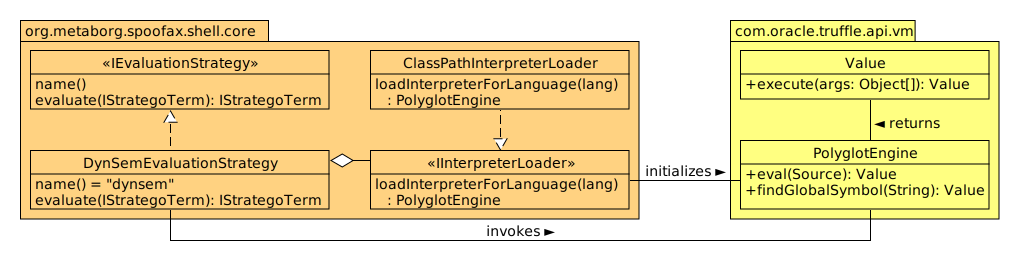
\includegraphics[width=\textwidth]{uml-dynsem-eval-strat}
  \caption{UML diagram of the \texttt{DynSemEvaluationStrategy} and its
    collaborator \texttt{IInterpreterLoader}.}
  \label{fig:uml-dynsem-eval-strat}
\end{figure}

%%% Local Variables:
%%% mode: latex
%%% TeX-master: "../main"
%%% End:
